\documentclass{article}

\usepackage[utf8]{inputenc}
\usepackage{amsmath}
\usepackage{adjustbox}
\usepackage{amsfonts}
%\usepackage{txfonts}

\usepackage[a4paper, total={150mm,247mm}]{geometry}

\newcommand{\R}{{\rm I\!R}}
\newcommand{\N}{{\rm I\!N}}

\begin{document}
%
\title{Wavelet Kompression und Multiskalenanalyse}
\author{Niklas Budinger \and Simon Cordes}
\maketitle

\section{Einleitung}
%
Auf dem Computer werden jegliche Informationen in Form von Bits, also Zahlenfolgen bestehend aus 0 und 1, gespeichert. Der Speicherplatz ist dabei beschränkt und es ist oft erstrebenswert die Menge an Bits, welche eine Information repräsentieren, zu reduzieren. Man unterscheidet dabei zwischen zwei Arten dieser sogenannten Kompression:\\
Bei der verlustfreien Kompression wird versucht die Entropie der Zahlenfolge, welche die Information repräsentiert, zu maximieren, um so den selben Informationsgehalt auf weniger Bits zu verteilen.
Höhere Kompressionsgrade erhält man hingegen mit verlustbehafteter Kompression. Dabei wird das Informationsgut in Klassen verschiedener Wichtigkeit aufgeteilt, um so von einem bestimmten Grad an Details -- im Tausch gegen reduzierten Speicherbedarf -- absehen zu können. Eine Methode zur Aufteilung der Informationen in Detailstufen ist die Wavelet-Transformation. Neben der Kompression kommt sie auch bei graphischen Anwendungen zum Einsatz.\\
Es sollen hier nun das mathematische Grundgerüst der Wavelet-Transformation, die Multiskalenanalyse, sowie die Bildkompression am Beispiel von Haar-Wavelets, und graphische Anwendungen am Beispiel von B-Splines vorgestellt werden.
% !TeX spellcheck = de_DE
\section{Multiskalenanalyse}
%
Das mathematische Äquivalent der Beschreibung eines Objektes mithilfe von Koeffizienten ist ein Vektorraum. Jedes Element des Vektorraums kann dabei bei gegebener (Schauder-)Basis als eine endliche bzw. abzählbar unendliche Folge von Koeffizienten dargestellt werden. Wir wollen uns hier, den später präsentierten Anwendungen entsprechend, auf endlich-dimensionale Vektorräume beschränken.

\subsection{Mathematische Konstruktion}
Es bezeichne $\Phi^N=\{\phi^N_1, ..., \phi^N_{\dim V_N}\}$ die zu den gespeicherten Koeffizienten gehörige Basis und $V_N:=\mathrm{span}(\Phi^N)$ den zugehörigen Vektorraum.\\
Für die Multiskalenanalyse wird nun ein Set von geschachtelten Vektorräumen\begin{equation*}
V_0\subset V_1\subset V_2\subset ...\subset V_{N-1}\subset V_N
\end{equation*}mit zugehörigen Basen\begin{equation*}
\Phi^i=\{\phi^i_1, ..., \phi^i_{\dim V_i}\}
\end{equation*}benötigt. Die Wahl eines Skalarproduktes über $V_N$ fixiert dann die orthogonalen Komplemente der $V_i$:\begin{equation*}
W_i:=V_i^\perp \mathrm{\ \ in\ \ } V_{i+1}\qquad\Leftrightarrow\qquad W_i\oplus V_i=V_{i+1}
\end{equation*}Die induzierte Norm übernimmt dabei die Rolle eines Fehlermaßes, dies sollte bei der Wahl des Skalarproduktes bedacht werden.
Nun müssen noch die Basisvektoren der orthogonalen Komplemente gewählt werden:\begin{equation*}
\Psi^i=\{\psi^i_1, ..., \psi^i_{\dim W_i}\}
\end{equation*}Die $\phi^i_j$s werden als Skalenfunktionen, die $\psi^i_j$s als Wavelets (von englisch wave: Welle und französisch -lette: klein) bezeichnet.\\
Standardmäßig werden Funktionen des $\mathcal{L}^2([0,1])$ unter dem Standardskalarprodukt\begin{equation*}
\left\langle f\mid g\right\rangle :=\int_{0}^{1}f(x)\cdot g(x)\mathrm{d}x
\end{equation*}betrachtet. Um eine gleichmäßige Informationsdichte zu ermöglichen werden die Skalenfunktionen dann ihrem Namen entsprechend als skalierte und verschobene Versionen der $V_0$-Basisvektoren gewählt:\begin{equation*}
\phi^i_{k\cdot j}(x)=\begin{cases}
\phi^0_j(m^i x-(k-1)),&m^i x-(k-1)\in[0,1]\\
0, &\mathrm{sonst}
\end{cases};\qquad 1\leq k\leq m^i, \ \ m\in \mathbb{N}.
\end{equation*}Der Skalierungsfaktor $m$ legt dabei die Vektorraumdimensionen fest:\begin{equation*}
\dim V_i=m^i\cdot \dim V_0;\qquad\dim W_i=(m-1)m^i\cdot \dim V_0
\end{equation*}Auch die Wavelets können dann als skalierte und verschobene Versionen der $\{\Psi^0\}$ gewählt werden. Es ist meist erstrebenswert, dass sie eine Orthonormalbasis der $W_i$ bilden, einen kleinen Träger besitzen und bis zu einem gewissen Maße stetig differenzierbar sind. Wavelets welche alle drei Eigenschaften erfüllen sind als Daubechies-Wavelets bekannt.

\subsection{Die Filter Bank}
Die Konstruktion der orthogonalen Komplemente $W_i$ erlaubt es nun die Elemente jedes Vektorraums $V_i=V_{i-1}\oplus W_{i-1}$ in der Basis $\{\phi^{i-1}_1, ..., \phi^{i-1}_{\dim V_{i-1}}, \psi^{i-1}_1, ..., \psi^{i-1}_{\dim W_{i-1}}\}$ darzustellen. Die Basistransformationsmatrix $T^i_{sf\rightarrow wl}$ ist mit der Wahl der Basisvektoren eindeutig festgelegt durch\begin{equation*}
\left[ \Phi^i\right] =\left[ \Phi^{i-1}\mid \Psi^{i-1}\right] \cdot T^i_{sf\rightarrow wl}=:\left[ \Phi^{i-1}\mid \Psi^{i-1}\right]\left[ \frac{\ A^i\ }{\ B^i\ }\right].
\end{equation*}Die Matrizen $A^i$ und $B^i$ sind einzeln betrachtet Projektionen, welche $V_i$ auf die Unterräume $V_{i-1}$ bzw. $W_{i-1}$ abbilden. Sie werden als Analyse-Filter bezeichnet. Die Rücktransformation ist gegeben durch\begin{equation*}
T^i_{wl\rightarrow sf}=\left[ \frac{\ A^i\ }{\ B^i\ }\right]^{-1}=:\left[ P^i\mid Q^i\right].
\end{equation*}Die Matrizen $P^i$ und $Q^i$ werden dabei als Synthese Filter bezeichnet.\\
Ist nun ein Koeffizientenvektor $C^i$ zur Basis $\Phi^i$ gegeben, so erhalten wir die Koeffizienten $C^{i-1}$ des Unterraums zur Basis $\Phi^{i-1}$ und die Detailkoeffizienten $D^i$ zur Wavelet-Basis $\Psi^i$ durch\begin{equation*}
	\begin{cases}
	&A^i\cdot C^i=C^{i-1}\\
	&B^i\cdot C^i=D^{i-1}.
	\end{cases}
\end{equation*}
Um die Elemente des $V_N$ in der Basis des $V_0\oplus W_0 \oplus...\oplus W_{N-1}$ also komplett mithilfe der Wavelets darzustellen, werden nun die Analyse Filter rekursiv angewendet. Dieser Prozess wird Filter Bank genannt.
\begin{figure}[h]
	\centering
	\includegraphics[page=11, trim=60 695 305 100, clip, width=0.7\textwidth]{4_wavelet_final[14255].pdf}
	\caption{Die Filter Bank}
\end{figure}\\
Werden nun in dieser Wavelet-Basis Koeffizienten weggelassen, erhalten wir nicht mehr ein unvollständiges Bild (bzw. Vektorraumelement), sondern ein niedriger aufgelöstes Bild (bzw. Element eines skalierten Unterraums). Bevor wir uns mit der Kompression beschäftigen, wollen wir allerdings zuerst als einfachstes und doch praktisches Beispiel die Haar-Wavelets einführen.


\section{Haar-Wavelets}

Die Haar-Skalenfunktionen und -Wavelets sind nur stückweise stetige Funktionen auf $\mathcal{L}^2([0,1])$ bzw. $\mathcal{L}^2([0,1])\times\mathcal{L}^2([0,1])$. Dafür bilden sie eine Orthonormalbasis, besitzen einen kleinen Träger und sind insgesamt sehr einfach zu handhaben. Die Skalenfunktionen entsprechen dabei den einzelnen Pixeln eines Bildes, während die Wavelets die Differenz benachbarter Pixel darstellen. Die zweidimensionale Variante ist somit für eine beispielhafte Anwendung der Bildkompression hervorragend geeignet. Zunächst sollen jedoch die eindimensionalen Haar-Wavelets eingeführt werden, um die Konstruktion ihres zweidimensionalen Äquivalents zu erleichtern.

\subsection{1D Haar-Wavelets}
Die 1D Haar-Wavelets sind im Funktionenraum $\mathcal{L}^2([0,1])$ unter dem Standardskalarprodukt definiert.
Es ist ausreichend die zu skalierende Skalenfunktion $\phi^0$ und das zugehörige Wavelet $\psi^0$ anzugeben:\begin{align*}
	\phi^0(x) &= \chi_{[0,1)}(x)\\
	\psi^0(x) &= \chi_{[0,\frac{1}{2})}(x)-\chi_{[\frac{1}{2}, 1)}(x)
\end{align*}
Alle weiteren Skalenfunktionen und Wavelets werden durch die folgende Skalierung und Verschiebung erzeugt:\begin{align*}
	\phi^i_{k}(x)&=\begin{cases}
	\sqrt{2^i}\phi^0(2^i x-k)),&2^i x-k\in[0,1]\\
	0, &\mathrm{sonst}
	\end{cases};\qquad 0\leq k\leq 2^i-1\\
	\psi^i_{k}(x)&=\begin{cases}
	\sqrt{2^i}\psi^0(2^i x-k)),&2^i x-k\in[0,1]\\
	0, &\mathrm{sonst}
	\end{cases};\qquad 0\leq k\leq 2^i-1
\end{align*}Damit sind auch die geschachtelten Vektorräume $V^i_{1D}$, die orthogonalen Komplemente $W^i_{1D}$ und die Analyse und Synthese Filter $A^i$, $B^i$, $P^i$ sowie $Q^i$ festgelegt und auch leicht zu bestimmen.
\begin{figure}[h]
	\centering
	\includegraphics[page=3, trim=166 490 346 276, clip, width=0.3\textwidth]{4_wavelet_final[14255].pdf}
	\includegraphics[page=3, trim=141 187 365 570, clip, width=0.3\textwidth]{4_wavelet_final[14255].pdf}
	\caption{Skalenfunktionen (links) und Wavelet-Basis (rechts) des $V_{1D}^3$}
\end{figure}

\subsection{2D Haar-Wavelets}
Die 2D Haar-Wavelets sind im Funktionenraum $\mathcal{L}^2([0,1])\times\mathcal{L}^2([0,1])$ unter folgendem Skalarprodukt definiert:\begin{equation*}
	\left\langle f, g\right\rangle _{2D}:=\int_{0}^{1}\int_{0}^{1}f(x,y)g(x,y)\mathrm{d}x\mathrm{d}y
\end{equation*}
Die geschachtelten Vektorräume sowie Skalenfunktionen werden als kartesisches Produkt zweier eindimensionaler Haar-Räume bzw. Skalenfunktionen gesetzt:\begin{align*}
	V^i_{2D}&:= V^i_{1D}\times V^i_{1D}\\
	\Phi^i_{2D}(x, y)&:=\{\phi^i_k(x)\phi^i_l(y)\mid \phi^i_k, \phi^i_l\in\Phi^i_{1D} \}
\end{align*}
Für die Konstruktion der Wavelets gibt es zwei gängige Varianten:
\paragraph{Standard-Konstruktion}~\\
Hierbei wird die 1D Wavelet-Basis $\Phi_{1D}^0\cup\Psi_{1D}^0\cup...\cup\Psi_{1D}^{i}$ für x- und y-Achse separat angewandt:\begin{align*}
	\Psi^i_{2D}(x, y)&:=\{\psi^i_k(x)\lambda^i_l(y)\mid \psi^i_k\in\Psi_{1D}^{i};\lambda^i_l\in\Phi_{1D}^0\cup\Psi_{1D}^0\cup...\cup\Psi_{1D}^{i} \}\\
	&\cup\ \{\lambda^i_k(x)\psi^i_l(y)\mid \psi^i_l\in\Psi_{1D}^{i};\lambda^i_k\in\Phi_{1D}^0\cup\Psi_{1D}^0\cup...\cup\Psi_{1D}^{i} \}
\end{align*}Bildlich gesprochen wird die 1D Wavelet-Transformation zuerst auf die Zeilen angewendet, um dann die erhaltenen transformierten Koeffizienten spaltenweise einer zweiten 1D Wavelet-Transformation zu unterziehen.
\paragraph{Nicht-Standard-Konstruktion}~\\
Bei der Nicht-Standard-Konstruktion werden als Ausgangspunkt die Wavelets $\Psi^0_{2D}$ der Standard-Konstruktion verwendet und in x- und y-Richtung gleichzeitig skaliert:\begin{equation*}
	\tilde\Psi^i_{2D}(x, y):=\{2^i\psi^0(2^ix-k, 2^iy-l)\mid \psi^0 \in \Psi^0_{2D}\}
\end{equation*}Bildlich werden ebenfalls nacheinander 1D Wavelet-Transformationen auf Zeilen und Spalten angewendet, allerdings abwechselnd.
\begin{figure}[h]
	\centering
	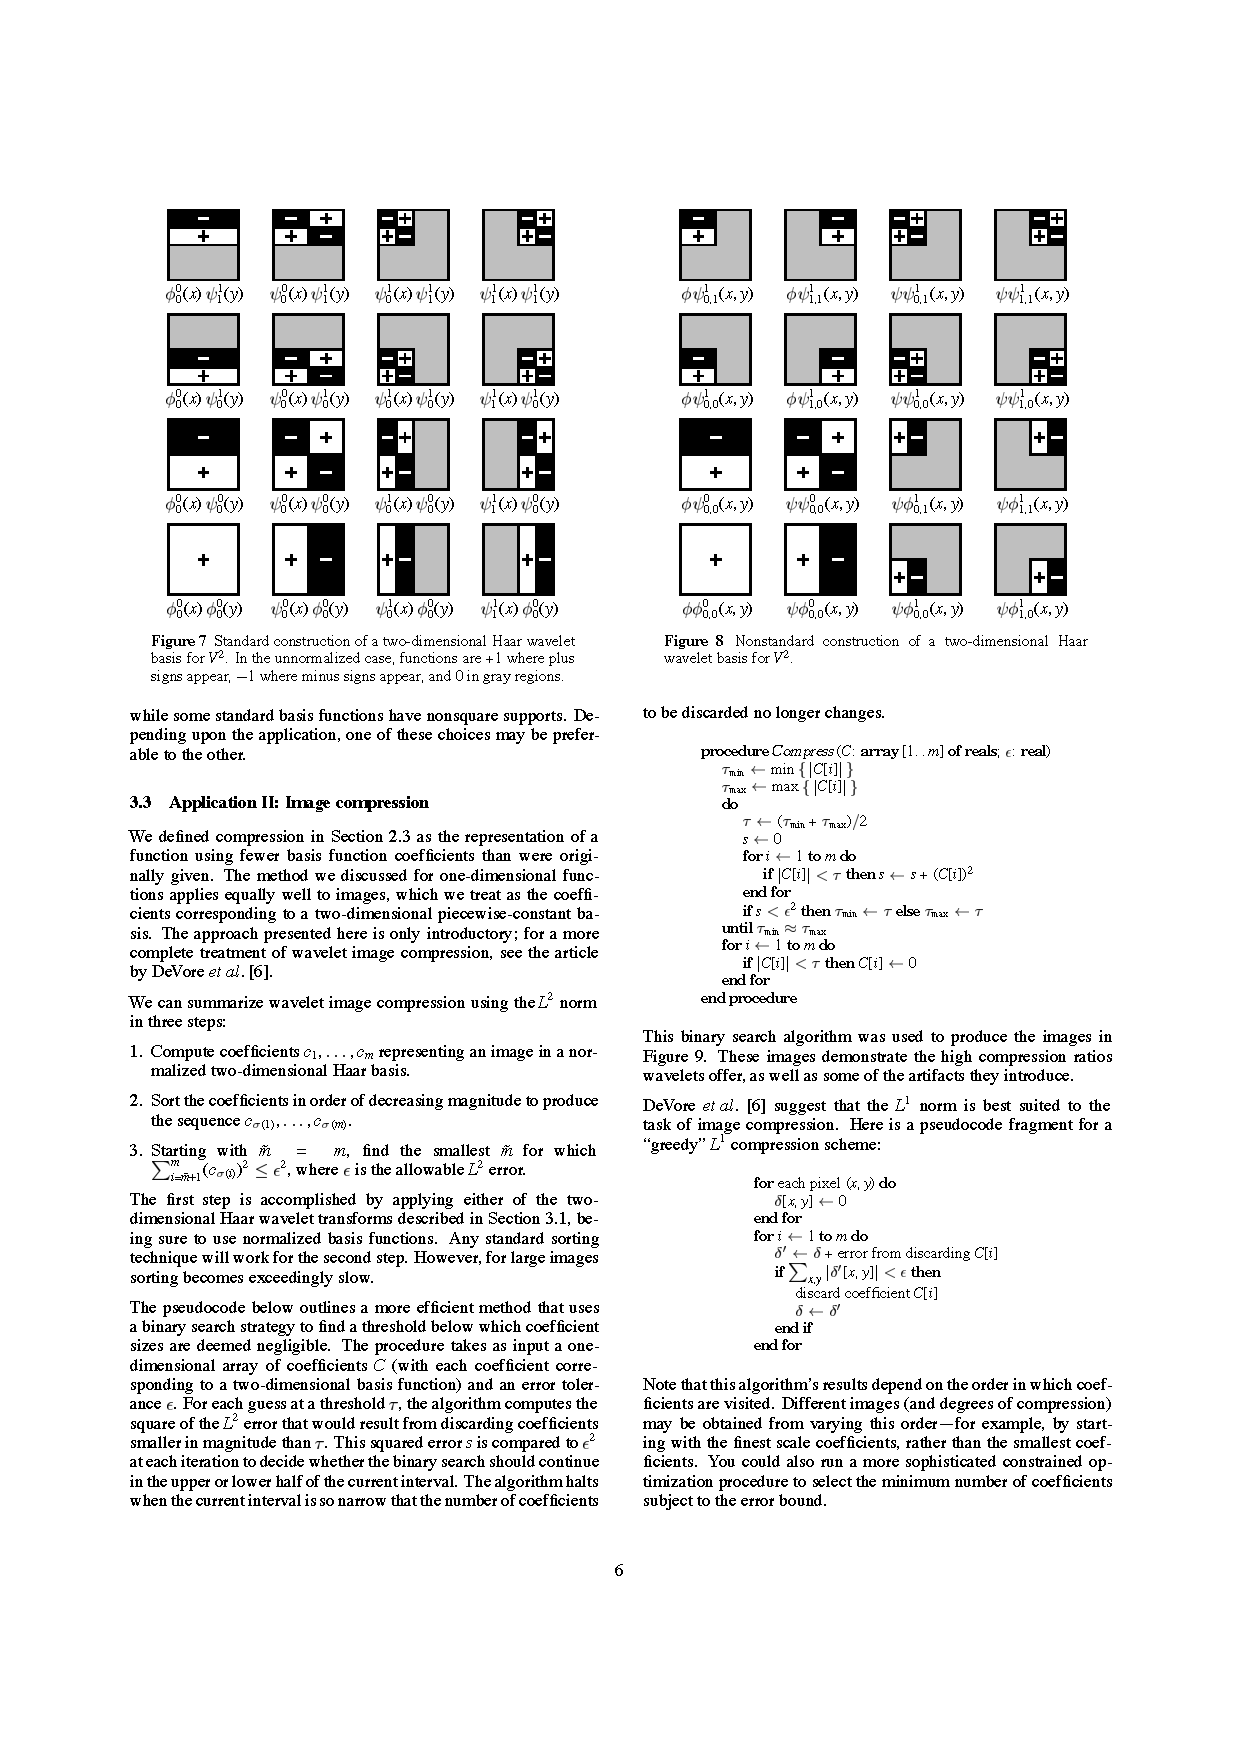
\includegraphics[trim=79 545 300 100, clip, width=0.45\textwidth]{2d_wavelets.pdf}
	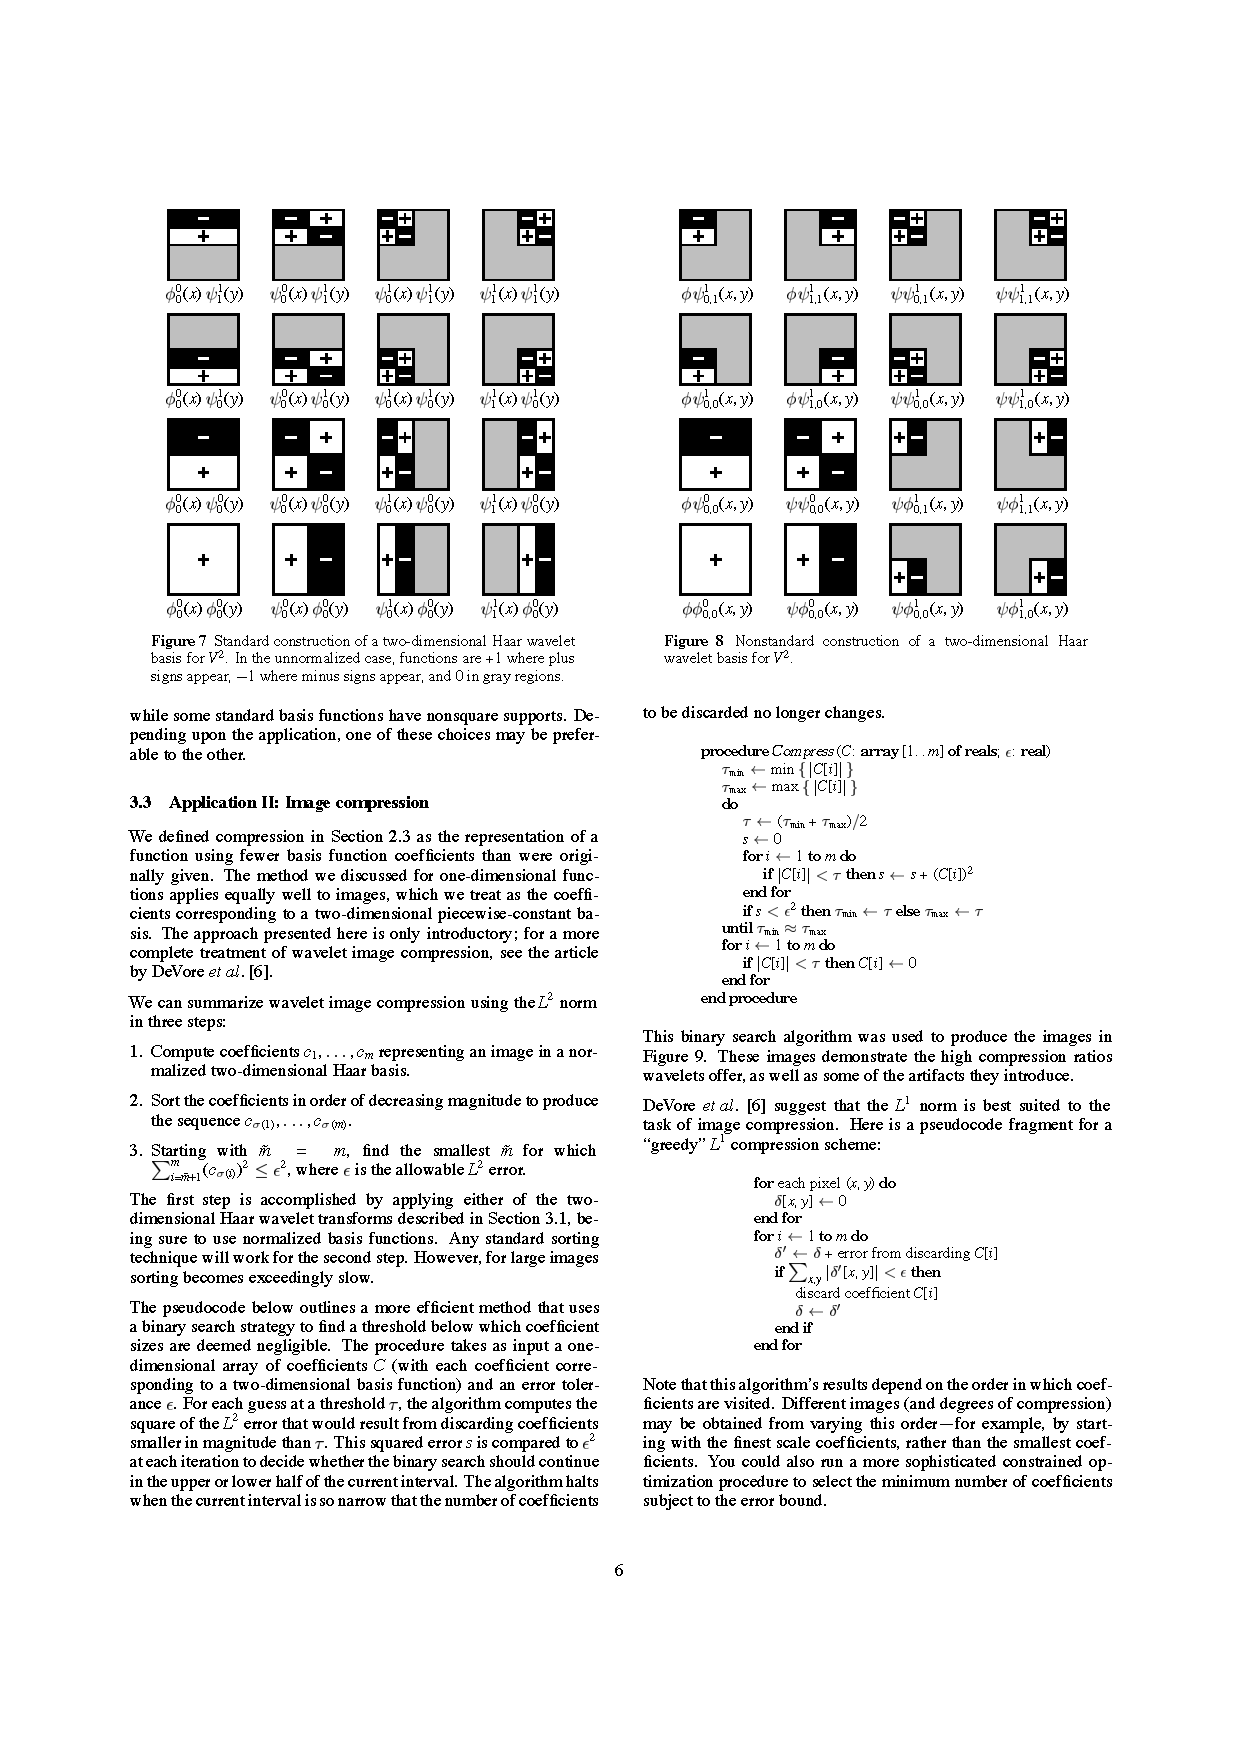
\includegraphics[trim=300 545 79 100, clip, width=0.45\textwidth]{2d_wavelets.pdf}
	\caption{2D Haar-Wavelets des $V_{2D}^3$: Standard-Konstruktion (links) und Nicht-Standard-Konstruktion (rechts)}
\end{figure}\\
Vorteil der Standard-Konstruktion ist die Möglichkeit nur 1D Wavelet-Transformation implementieren zu müssen, Nachteil ist ein etwas höherer Rechenaufwand. Außerdem unterscheiden sich beide Konstruktionen bezüglich der Form der Träger: Während die Nicht-Standard-Konstruktion ausschließlich Wavelets mit quadratischen Trägern hervorbringt, haben die Wavelets nach Standard-Konstruktion zu Teilen rechteckige Träger. Welche Methode besser geeignet ist, hängt somit vor allem von der Anwendung ab.
	

\section{Anwendungen}
%
\subsection{Bildkompression}
%
\subsubsection{Algorthimen für Haar-Analyse und Synthese}
%
\paragraph{1D Signale}~\\
Nun geht es um die konkrete Realisierung einer Filterbank für Analyse und Synthese von Signalen. Da es sich bei der Haar-Basis um eine Orthonormalbasis handelt, läge es auf Anhieb nahe, die Koeffizienten einfach über ein Skalarprodukt mit der entsprechenden Basisfunktion zu berechnen. Da alle betracheten Funktionen stückweise konstant sind, wäre ein solches Vorgehen prinzipiell machbar, es stellt sich aber heraus, dass man auf diese Weise einige Zwischneergebnisse mehrfach berechnet, was eine relative hohe Laufzeit zur Folge hat. Einen effizienteren Algorithmus erhält man, indem man sich stärker an den konzeptionellen Ablauf der Filterbank hält und das Signal schrittweise analysiert.\\
%
Die Approximation eines Signales liege in Form einer Liste $C$ von $2^j$ Koeffizienten bezüglich der Skalierungsfunktionenbasis des Raumes $V^j = V^{j-1} \oplus W^{j-1}$ vor. Ein Schritt des zu implementierenden Filterbank-Algorithmus erhälte nun eine solche Liste $C$ und führte eine Basistransformation durch, sodass eine Liste $C'$ gleicher Länge entsteht, deren erste $2^{j-1}$ Einträge die Koeffizienten bezüglich der Skalierungsfunktionenbasis von $V^{j-1}$ darstellen, während die übrigen $2^{j-1}$ Einträge die Koeffizienten bezüglich der zugehörigen Waveletbasis von $W^{j-1}$ sind.\\
Die genaue Berechnungsvorschrift hierfür erhält man aus den Beziehungen der Skalierungsfunktionen $(\phi_{i}^{j-1})_{i=0}^{2^{j-1}-1}$ und Waveletfunktionen $(\psi_{i}^{j-1})_{i=0}^{2^{j-1}-1}$ auf Level $(j-1)$ und den Skalierungsfunktionen $(\phi_{i}^{j})_{i=0}^{2^{j}-1}$ auf Level $j$. Für $i = 0, 1, ..., 2^{j-1}-1$ gilt:
%
\[
\phi_{i}^{j-1} = \frac{1}{\sqrt{2}}( \phi_{2i}^{j} + \phi_{2i+1}^{j} )
\qquad , \qquad
\psi_{i}^{j-1} = \frac{1}{\sqrt{2}}( \phi_{2i}^{j} - \phi_{2i+1}^{j} )
,
\]
oder in Matrixschreibweise:
\[
\left[ \phi\psi \right]_{i}^{j-1}
:=
\begin{pmatrix}
\phi_{i}^{j-1} \\
\psi_{i}^{j-1}
\end{pmatrix}
=
\frac{1}{\sqrt{2}}
\begin{pmatrix}
1 & 1 \\
1 & -1
\end{pmatrix}
\begin{pmatrix}
\phi_{2i}^{j} \\
\phi_{2i+1}^{j}
\end{pmatrix}
=:
\mathbf{M}
\begin{pmatrix}
\phi_{2i}^{j} \\
\phi_{2i+1}^{j}
\end{pmatrix}
=:
\mathbf{M}
\left[ \phi\phi \right]_{i}^j
.
\]
%
(\textbf{BILD!!!}) Diese Beziehungen leifern eine vollständige Charakterisierung des Basiswechsels, aus ihnen ließen sich zum Beispiel auch die Synthesematrizen $\mathbf{P}^j$ und $\mathbf{Q}^j$ aus der theoretischen Behandlung ableiten.\\
Wie man leicht sieht, ist die Matrix $\mathbf{M}$ selbstinvers. Für die umgekehrte Beziehung erhält man folglich für $i = 0, 1, ..., 2^{j-1}-1$ ebenfalls:
%
\[
\left[ \phi\phi \right]_{i}^j
=
\mathbf{M}
\left[ \phi\psi \right]_{i}^{j-1}
.
\]
%
Die Koeffiziententransformation ist daher für einen Analyse-Schritt bzw. für einen Synthese-Schritt in beiden Fällen die selbe, nämlich eine Rechtsmultiplikation mit $\mathbf{M}$, denn für $i = 0, 1, ..., 2^{j-1}-1$ gilt:
%
\[
\begin{pmatrix}
a & b
\end{pmatrix}
\left[ \phi\psi \right]_{i}^{j-1}
=
\underbrace{
\begin{pmatrix}
a & b
\end{pmatrix}
\mathbf{M}
}_{
\begin{pmatrix}
a' & b'
\end{pmatrix}
}
\left[ \phi\phi \right]_{i}^j
\qquad \mbox{und} \qquad
\begin{pmatrix}
a' & b'
\end{pmatrix}
\left[ \phi\phi \right]_{i}^j
=
\underbrace{
\begin{pmatrix}
a' & b'
\end{pmatrix}
\mathbf{M}
}_{
\begin{pmatrix}
a & b
\end{pmatrix}
}
\left[ \phi\psi \right]_{i}^{j-1}
\]
%
\[
\mbox{mit} \qquad \qquad
\begin{pmatrix}
x & y
\end{pmatrix}
\mathbf{M}
=
\begin{pmatrix}
\frac{x+y}{\sqrt{2}} & \frac{x-y}{\sqrt{2}}
\end{pmatrix}
.
\]
%
Konkret folgen hieraus für einen Analyse-Schritt des Filterbank-Algorithmus und den inversen Synthese-Schritt die folgenden Implementierungen der Basiswechsel. $C$ und $C'$ sind dabei Listen von Koeffizienten, wie sie weiter oben eingeführt wurden.

\begin{adjustbox}{max width=\textwidth ,center}
\begin{tabular}{p{.575\textwidth}|p{.575\textwidth}}
\begin{verbatim}
def analysisStep(C):
    C' = empty_like(C)
    h = C.size // 2
    for i in range(h):
        C'[i] = (C[2*i] + C[2*i+1])/sqrt(2)
        C'[h+i] = (C[2*i] - C[2*i+1])/sqrt(2)
    return C'
\end{verbatim}
&
\begin{verbatim}
def synthesisStep(C'):
    C = empty_like(C')
    h = C'.size // 2
    for i in range(h):
        C[2*i] = (C'[i] + C'[h+i])/sqrt(2)
        C[2*i+1] = (C'[i] - C'[h+i])/sqrt(2)
    return C
\end{verbatim}
\\
\end{tabular}
\end{adjustbox}

\noindent Eine vollständige Wavelet-Transformation erhält man dann durch rekursive Analyse der $\phi^{j}$-Koeffizienten, die Rücktransformation entsprechend durch widerholte Synthese-Schritte:

\begin{adjustbox}{max width=\textwidth ,center}
\begin{tabular}{p{.575\textwidth}|p{.575\textwidth}}
\begin{verbatim}
def analysis(C):
    C' = copy(C)
    h = C.size
    while h > 1:
        C' = analysisStep(C'[0:h])
        h = h // 2
    return C'
\end{verbatim}
&
\begin{verbatim}
def synthesis(C'):
    C = copy(C')
    h = 1
    while h < C'.size:
        h = 2*h
        C = synthesisStep(C[0:h])
    return C
\end{verbatim}
\\
\end{tabular}
\end{adjustbox}

\noindent \textbf{Zur Laufzeit:} Ein Analyse- bzw. Synthese-Schritt eines Signals der Länge $m$ benötigt von der Größenordnung $m$ Operationen innerhalb der Schleife. Für eine vollständige Analyse bzw. Synthese eines Signals der Länge $n=2^k$ werden $k$ Teilschritte zu den Teillängen $2^k, 2^{k-1}, ... 2^2, 2$ durchgeführt. Die Gesamtkomplexität beläuft sich damit auf $\sum_{i=1}^k 2^i = 2^{k+1}-2 = (2n-2)$ Operationen.
%
\paragraph{2D Signale bzw. Bilder}~\\
Für 2D Signale muss zwischen der Standard- und der Nicht-Standard-Basis unterschieden werden. Für beide sind Analyse und Synthese allerdings relativ einfach zu Implementieren und bauen auf den Algorithmen für den eindimensionalen Fall auf.

\subparagraph{Standard-Basis} Die Analyse bzgl. der Standard-Basis, welche aus den Tensorprodukten der eindimensionalen Skalieungsfunktionen und Wavelets aufgebaut ist, kann in zwei Schritten mit Hilfe der eindimensionalen Analyse durchgeführt werden. Die Idee dahinter ist, die Analyse erst bezüglich der einen Achse und danach bezüglich der anderen Achse durchzuführen.
%
\[
\begin{array}{ccc}
{
\begin{array}{cccc}
\phi_0^0(x)\phi_0^0(y) & \phi_0^1(x)\phi_0^0(y) & \phi_1^1(x)\phi_0^0(y) & \hdots \\
\phi_0^0(x)\phi_0^1(y) & \phi_0^1(x)\phi_0^1(y) & \phi_1^1(x)\phi_0^1(y) & \hdots \\
\phi_0^0(x)\phi_1^1(y) & \phi_0^1(x)\phi_1^1(y) & \phi_1^1(x)\phi_1^1(y) & \hdots \\
\vdots & \vdots & \vdots & \ddots \\
\end{array}
} &
\overset{\mbox{\small \textbf{I}}}{\longrightarrow} &
{
\begin{array}{cccc}
\phi_0^0(x)\phi_0^0(y) & \psi_0^0(x)\phi_0^0(y) & \psi_0^1(x)\phi_0^0(y) & \hdots \\
\phi_0^0(x)\phi_0^1(y) & \psi_0^0(x)\phi_0^1(y) & \psi_0^1(x)\phi_0^1(y) & \hdots \\
\phi_0^0(x)\phi_1^1(y) & \psi_0^0(x)\phi_1^1(y) & \psi_0^1(x)\phi_1^1(y) & \hdots \\
\vdots & \vdots & \vdots & \ddots \\
\end{array}
} \\
 &
 &
\big\downarrow \mbox{\small \textbf{II}} \\[.25cm]
 &
 &
{
\begin{array}{cccc}
\phi_0^0(x)\phi_0^0(y) & \psi_0^0(x)\phi_0^0(y) & \psi_0^1(x)\phi_0^0(y) & \hdots \\
\phi_0^0(x)\psi_0^0(y) & \psi_0^0(x)\psi_0^0(y) & \psi_0^1(x)\psi_0^0(y) & \hdots \\
\phi_0^0(x)\psi_0^1(y) & \psi_0^0(x)\psi_0^1(y) & \psi_0^1(x)\psi_0^1(y) & \hdots \\
\vdots & \vdots & \vdots & \ddots \\
\end{array}
}
\end{array}
\]
%
Jede Zeile des Bildes wird dabei zunächst als eindimensionales Signal interpretiert. Eine Separate Transormation der Zeilen entspricht dann dem Basiswechsel \textbf{I}. Interpretiert man nun jede Spalte des so transformierten Bildes als eindimensionales Signal und führt für jede Spalte separat eine Transformation durch, so entspricht dies dem Basiswechsel \textbf{II}. Die Komposition von Basiswechsel \textbf{I} und \textbf{II} ergeben aber gerade einen Basiswechsel zur Standard-Haar-Wavelet-Basis. Entsprechend erhält man somit eine Algorithmus zum Durchführen der Analyse. Die Synthese funktioniert analog in umgekehrter Richtung. Man erhält:

\begin{adjustbox}{max width=\textwidth ,center}
\begin{tabular}{p{.575\textwidth}|p{.575\textwidth}}
\begin{verbatim}
def standardAnalysis(C):
    C' = copy(C)
    for i in range(C.shape[0]):
        C'[i,:] = analysis(C'[i,:])
    for j in range(C.shape[1]):
        C'[:,j] = analysis(C'[:,j])
    return C'
\end{verbatim}
&
\begin{verbatim}
def standardSynthesis(C'):
    C = copy(C')
    for j in range(C'.shape[1]):
        C[:,j] = synthesis(C[:,j])
    for i in range(C'.shape[0]):
        C[i,:] = synthesis(C[i,:])
    return C
\end{verbatim}
\\
\end{tabular}
\end{adjustbox}

\noindent Für ein Bild mit $n \times n$ Pixeln werden in Analyse und Synthese zweimal je $n-$mal die eindimensionnale Analyse und Synthese aufgerufen. Die Komplexität der Operationen liegt daher je bei $n(2n-2) + n(2n-2) = 4n^2-4n$.

% Ich bin mit dieser Abhandlung noch nicht wirklich zufrieden.... aber es sollte wohl reichen.....
% Was irgendwie noch fehlt ist eine Behandlung der eigendlichen n x n Koeffizientenlisten, welche
% sukzessive transformiert werden. Ich denke, dieser Aspekt sollte ein zentraler Punkt im Vortrag 
% werden. Wenn ich mir diesbezüglich etwas Schönes ausgedacht haben, kann ich es hier vielleicht noch
% einbringen...
\subparagraph{Nicht-Standard-Basis} Für die Nicht-Standard-Basis ist die Situation ein wenig komplizierter. Es stellt sich aber heraus, dass auch hier ein Teil der Routinen aus dem eindimensionalen Fall wiederverwendet werden können. Ausgangspunkt ist in diese Fall eine zweidimensionale $n \times n$ Liste $C$ von Koeffizienten bezüglich der $n^2$ Basisfunktionen, Ziel ist ein Basiswechsel in die Nicht-Standard-Haar-Wavelet-Basis.\\
Wie im eindimensionalen Fall steht zu Beginn die Beziehung zwischen den Skalierungsfunktionen auf Level $j$ und den Skalierungsfunktionen und Wavelets auf Level $(j-1)$. Hier gilt für $k, l = 0, 1, ..., 2^{j-1}-1$:
%
\[
\left[ \phi\psi \right]_{k,l}^{j-1}
:=
\begin{pmatrix}
\phi\phi_{k,l}^{j-1} \\
\psi\phi_{k,l}^{j-1} \\
\phi\psi_{k,l}^{j-1} \\
\psi\psi_{k,l}^{j-1} \\
\end{pmatrix}
= \frac{1}{2}
\begin{pmatrix}
1 & 1 & 1 & 1 \\
1 & -1 & 1 & -1 \\
1 & 1 & -1 & -1 \\
1 & -1 & -1 & 1 \\
\end{pmatrix}
\begin{pmatrix}
\phi\phi_{2k,2l}^{j} \\
\phi\phi_{2k+1,2l}^{j} \\
\phi\phi_{2k,2l+1}^{j} \\
\phi\phi_{2k+1,2l+1}^{j} \\
\end{pmatrix}
=:
\mathbf{M}
\begin{pmatrix}
\phi\phi_{2k,2l}^{j} \\
\phi\phi_{2k+1,2l}^{j} \\
\phi\phi_{2k,2l+1}^{j} \\
\phi\phi_{2k+1,2l+1}^{j} \\
\end{pmatrix}
=:
\mathbf{M}
\left[ \phi\phi \right]_{k,l}^j
\]
%
Dieser Zusammenhang ist einfacher zu verstehen, wenn man eine etwas andere Schreibweise einführt. Genauer wird eine alternative Schreibweise für Koeffizienten-Spaltenvektoren verwendet, bei der die Anordnung der Einträge ihrer relativen Position in der zweidimensionalen Koeffizientenliste $C$ entspricht:
%
\[
\begin{array}{c|c}
a & b \\[.05cm] 
\hline \\[-0.35cm]
c & d
\end{array}
:=
\begin{pmatrix}
a & b & c & d
\end{pmatrix}
\qquad \mbox{, sodass} \qquad
\begin{pmatrix}
a & b & c & d
\end{pmatrix}
\left[ \phi\phi \right]_{k,l}^j
=
\begin{array}{c|c}
a & b \\[.05cm] 
\hline \\[-0.35cm]
c & d
\end{array}
\left[ \phi\phi \right]_{k,l}^j
.
\]
%
Drückt man die obige Beziehung auf diese Weise aus, so erhält man: \textbf{(Stelle sicher, dass die Darstellung konsistent ist!!!)}
%
\begin{align*}
\phi\phi_{k,l}^{j-1} &=
\frac{1}{2} \times
\begin{array}{c|c}
1 & 1 \\[.05cm] 
\hline \\[-0.35cm]
1 & 1
\end{array}
\left[ \phi\phi \right]_{k,l}^j
\quad , &
\psi\phi_{k,l}^{j-1} &=
\frac{1}{2} \times
\begin{array}{c|c}
1 & -1 \\[.05cm] 
\hline \\[-0.35cm]
1 & -1
\end{array}
\left[ \phi\phi \right]_{k,l}^j
\quad , \\
\phi\psi_{k,l}^{j-1} &=
\frac{1}{2} \times
\begin{array}{c|c}
1 & 1 \\[.05cm] 
\hline \\[-0.35cm]
-1 & -1
\end{array}
\left[ \phi\phi \right]_{k,l}^j
\quad , &
\psi\psi_{k,l}^{j-1} &=
\frac{1}{2} \times
\begin{array}{c|c}
1 & -1 \\[.05cm] 
\hline \\[-0.35cm]
-1 & 1
\end{array}
\left[ \phi\phi \right]_{k,l}^j
\quad .
\end{align*}
%
Stellt man nun fest, dass die Anordnung der Koeffizienten gerade der Anordung der Träger der Einträge von $\left[ \phi\phi \right]_{k,l}^j$ entspricht, so ergibt sich die Beziehung anschaulich aus der Form der dargestellten Funktionen.\\
%
Wie man leicht nachprüft ist die Matrix $\mathbf{M}$ wieder selbsinvers. Analog zum eindimensionalen Fall ergibt sich somit eine symmetrische Koeffiziententransformation durch Rechtsmultiplikation mit $\mathbf{M}$:
%
\[
\begin{array}{c|c}
a & b \\[.05cm] 
\hline \\[-0.35cm]
c & d
\end{array}
\left[ \phi\psi \right]_{k,l}^{j-1}
=
\underbrace{
\begin{array}{c|c}
a & b \\[.05cm] 
\hline \\[-0.35cm]
c & d
\end{array}
\mathbf{M}
}_{
\begin{array}{c|c}
a' & b' \\[.05cm] 
\hline \\[-0.35cm]
c' & d'
\end{array}
}
\left[ \phi\phi \right]_{k,l}^j
\qquad \mbox{und} \qquad
\begin{array}{c|c}
a' & b' \\[.05cm] 
\hline \\[-0.35cm]
c' & d'
\end{array}
\left[ \phi\phi \right]_{k,l}^{j}
=
\underbrace{
\begin{array}{c|c}
a' & b' \\[.05cm] 
\hline \\[-0.35cm]
c' & d'
\end{array}
\mathbf{M}
}_{
\begin{array}{c|c}
a & b \\[.05cm] 
\hline \\[-0.35cm]
c & d
\end{array}
}
\left[ \phi\psi \right]_{k,l}^{j-1}
\]
%
\[
\mbox{mit} \qquad \qquad
\begin{array}{c|c}
t & u \\[.05cm] 
\hline \\[-0.35cm]
v & w
\end{array}
\mathbf{M}
=
\frac{1}{2} \times
\begin{array}{c|c}
t+u+v+w & t-u+v-w \\[.05cm] 
\hline \\[-0.35cm]
t+u-v-w & t-u-v+w
\end{array}
.
\]
%
%\noindent Für $\mathbf{M}$ ergibt sich folgende Faktorisierung:
%
%\[
%\mathbf{M} = 
%\frac{1}{\sqrt{2}}
%\begin{pmatrix}
%1 & 1 & 0 & 0 \\
%1 & -1 & 0 & 0 \\
%0 & 0 & 1 & 1 \\
%0 & 0 & 1 & -1 \\
%\end{pmatrix}
%\frac{1}{\sqrt{2}}
%\begin{pmatrix}
%1 & 0 & 1 & 0 \\
%0 & 1 & 0 & 1 \\
%1 & 0 & -1 & 0 \\
%0 & 1 & 0 & -1 \\
%\end{pmatrix}
%=: \mathbf{M}_x \mathbf{M}_y
%\]
%
%\noindent Wie die Benennung suggestiert, handelt es sich bei $\mathbf{M}_x$ und $\mathbf{M}_y$ um 
%
%\begin{align*}
%\begin{pmatrix}
%a & b & c & d \\
%\end{pmatrix}
%\begin{pmatrix}
%\phi\phi_{k,l}^{j-1} \\
%\phi\psi_{k,l}^{j-1} \\
%\psi\phi_{k,l}^{j-1} \\
%\psi\psi_{k,l}^{j-1} \\
%\end{pmatrix}
%&= \frac{1}{2}
%\begin{pmatrix}
%a & b & c & d \\
%\end{pmatrix}
%\begin{pmatrix}
%1 & 1 & 1 & 1 \\
%1 & -1 & 1 & -1 \\
%1 & 1 & -1 & -1 \\
%1 & -1 & -1 & 1 \\
%\end{pmatrix}
%\begin{pmatrix}
%\phi\phi_{2k,2l}^{j} \\
%\phi\phi_{2k+1,2l}^{j} \\
%\phi\phi_{2k,2l+1}^{j} \\
%\phi\phi_{2k+1,2l+1}^{j} \\
%\end{pmatrix}
%\\
%&=
%\begin{pmatrix}
%\frac{a+b+c+d}{2} &
%\frac{a-b+c-d}{2} &
%\frac{a+b-c-d}{2} &
%\frac{a-b-c+d}{2} \\
%\end{pmatrix}
%\begin{pmatrix}
%\phi\phi_{2k,2l}^{j} \\
%\phi\phi_{2k+1,2l}^{j} \\
%\phi\phi_{2k,2l+1}^{j} \\
%\phi\phi_{2k+1,2l+1}^{j} \\
%\end{pmatrix}
%\end{align*}
%
$\mathbf{M}$ lässt sich in zwei kommutierende Matrizen $\mathbf{M}_x$ und $\mathbf{M}_y$ Faktorisieren. Wie die Bezeichnung suggestiert, handelt es sich dabei jeweils um einen Schritt der eindimensionalen Transformation, welche jeweils einmal entlang jeder Zeile des Koeffizientenfeldes für $\mathbf{M}_x$ und einmal entlang jeder Spalte für $\mathbf{M}_y$ durchgeführt wird:
%
\[
\begin{array}{ccc}
\begin{array}{c|c}
t & u \\[.05cm] 
\hline \\[-0.35cm]
v & w
\end{array}
&
\begin{array}{c}
 \\[-0.3cm] \mathbf{M}_x \\[-0.1cm] \longrightarrow \\ \\
\end{array}
&
\frac{1}{\sqrt{2}} \times
\begin{array}{c|c}
t\boldsymbol{+}u & t\boldsymbol{-}u \\[.05cm] 
\hline \\[-0.35cm]
v\boldsymbol{+}w & v\boldsymbol{-}w
\end{array}
\\[.5cm]
\big\downarrow \mathbf{M}_y & & \big\downarrow \mathbf{M}_y \\[.25cm]
\frac{1}{\sqrt{2}} \times
\begin{array}{c|c}
t\boldsymbol{+}v & u\boldsymbol{+}w \\[.05cm] 
\hline \\[-0.35cm]
t\boldsymbol{-}v & u\boldsymbol{-}w
\end{array}
&
\begin{array}{c}
 \\[-0.3cm] \mathbf{M}_x \\[-0.1cm] \longrightarrow \\ \\
\end{array}
&
\frac{1}{2} \times
\begin{array}{c|c}
(t+u)\boldsymbol{+}(v+w) & (t-u)\boldsymbol{+}(v-w) \\[.05cm] 
\hline \\[-0.35cm]
(t+u)\boldsymbol{-}(v+w) & (t-u)\boldsymbol{-}(v-w)
\end{array}
\\
\end{array}
\]
%
Das Resultat ist, dass ein Analyse-Schritt bezüglich der Nicht-Standard-Basis gerade ein Analyse-Schritt entlang einer Achse gefolgt von einem Analyse-Schritt entlang der anderen Achse ist. Selbiges gilt für die Synthese. Analog zum eindimensionalen Fall ergibt sich die Gesamtoperation für Analyse bzw. Synthese aus wiederholtem anwenden der Einzelschritte auf die Skalierungsfunktionskoeffizienten. Man erhält:

\begin{adjustbox}{max width=\textwidth ,center}
\begin{tabular}{p{.575\textwidth}|p{.575\textwidth}}
\begin{verbatim}
def nonstandardAnalysis(C):
    C' = copy(C)
    h = C.size
    while h > 1:
        for i in range(h):
            C'[i,0:h] = analysisStep(C'[i,0:h])
        for j in range(h):
            C'[0:h,j] = analysisStep(C'[0:h,j])
        h = h // 2
    return C'
\end{verbatim}
&
\begin{verbatim}
def nonstandardSynthesis(C'):
    C = copy(C')
    h = 1
    while h < C'.size:
        h = 2*h
        for j in range(h):
            C[0:h,j] = synthesisStep(C[0:h,j])
        for i in range(h):
            C[i,0:h] = synthesisStep(C[i,0:h])
    return C
\end{verbatim}
\\
\end{tabular}
\end{adjustbox}

\noindent Die Laufzeitkomplexität der Routinen für $n \times n$ Listen mit $n=2^k$ ergibt damit sich zu 
%
\[
\sum_{i=1}^k 2^i 2^i + 2^i 2^i
= \sum_{i=1}^k 2^{2i} + 2^{2i} 
= 2\sum_{i=1}^k 4^i 
= 8\sum_{i=0}^{k-1} 4^i 
= 8\frac{4^k-1}{4-1} 
= \frac{8}{3}((2^k)^2-1) 
= \frac{8}{3}(n^2-1)
.
\]
%
Die Nicht-Standard-Transformation ist somit etwas schneller als die Standard-Transformation.
%
% Wenn noch Zeit zu füllen ist, könnte es hier noch interessant sein zu zeigen, dass es auch 'Bilder'
% gibt, die sich auf diese Weise bezüglich der Haar-Basis nur schlecht komprimieren lassen.
% Eine solche Kompressionsstrategie kann immer nur für eine gewisse Klasse von Signalen funktionieren.
\subsubsection{Kompression}~\\
Das Ziel von Kompression ist die möglicherweise verlustbehaftete Darstellung eines Signals mit Hilfe möglichst weniger Bits. Im Folgenden soll auf einen möglichen Ansatz zum Erreichen dieses Ziels eingegangen werden.
Konkret werden hier Signale betrachtet, die sich als Elemente eines endlichdimensionalen Vektorraums mit einem Skalarprodukt, dessen induzierte Metrik ein passendes Maß für einen Approximationsfehler solcher Signale liefert, auffassen lassen. Wenn $m$ die Dimension dieses Vektorraumes ist, so werden im allgemeinen $m$ Koeffizienten bezüglich einer beliebigen Basis benötigt, um ein beliebiges Signal darzustellen. Ein einfacher Ansatz zur verlustbehafteten Kompression besteht darin, einige dieser Koeffizienten wegzulassen, d.h. auf Null zu setzen. Wie groß der hierdurch verursachte Approximationfehler ist, hängt im Allgemeinen nicht nur von der Größe der weggelassenen Koeffizienten, sondern auch von der gewählten Basis ab. Für Orthonoramalbasen ergibt sich ein besonders einfacher Zusammenhang: Sei $I=\{1,...,m\}$ die Indexmenge zum indizieren der Basis, $f=\sum_{i \in I} c_i \mathbf{b}_i$ ein Vektor representiert durch Koeffizienten $(c_i)$ bezüglich einer Orthonormalbasis $(\mathbf{b}_i)$ und $\tilde{f}=\sum_{i \in \tilde{I}} c_i \mathbf{b}_i$, wobei $\tilde{I} \subset I$, eine Approximation des Vektors. Der Approximationsfehler ergibt sich zu:
%
\[
||f-\tilde{f}||_2^2 
= \langle f-\tilde{f}, f-\tilde{f} \rangle 
= \langle \sum_{i \in (I \setminus \tilde{I})} c_i \mathbf{b}_i , \sum_{j \in (I \setminus \tilde{I})} c_j \mathbf{b}_j \rangle 
= \sum_{i,j \in (I \setminus \tilde{I})} c_i c_j \langle \mathbf{b}_i , \mathbf{b}_j \rangle 
= \sum_{i \in (I \setminus \tilde{I})} c_i^2
.
\]
%
Er hängt im Fall einer Orthonormalbasis also nur von der Größe der weggelassenen Koeffizienten ab. Für eine gegebene Klasse von Signalen, wie zum Beispiel Bildern, besteht die eigendliche Problemstellung für das Implementieren eines solchen Kompressionsalgorithmus in der Wahl einer Orthogonalbasis des Signalraumes, bezüglich der möglichst viele Koeffizienten betragsklein sind.\\
Für natürliche Bilder stellt sich heraus, dass die Haar-Basis der Wavelet-Transformation eine solche Rolle einnimmt. In anderen Worten: Die Haar-Wavelet-Transformation eines natürlichen Bildes weist in den meisten Fällen viele betragskleine Einträge auf. Da es sich bei der Haar-Basis um eine Orthonormalbasis handelt, bedeutet dies, dass hohe Kompressionsraten bei vergleichsmäßig geringem Approximationsfehler durch Weglassen der Betragskleinsten Koeffizienten möglich sind. \\
Der Konzeptionell einfachste Algorithmus hierzu besteht schlicht darin die Koeffizienten der Wavelet-Transformation absteigend zu sortieren. Ist eine gewisse Kompressionsrate gefordert, so lässt man einfach entsprechend viele Koeffizienten vom Ende der Liste weg. Ist ein gewisser Approximationsfehler einzuhalten, so lässt man gerade so viele Koeffizienten vom Ende der Liste weg, dass die Summe der Quadrate dieser noch unterhalb der quadrierten Fehlertolleranz liegt.
%

\subsection{Multiskalen-Representation von Splinekurven}
%
%\paragraph{}
%Im Fall von eindimensionalen Signalen oder zweidimensionalen Bildern ist es relativ intuitiv das Signal auf verschiedene Größenskalen darzustellen, man würde vermutlich auch ohne den theoretischen Rahmen der Multiskalenanalyse auskommen. Für abstraktere Anwendungen ist das hergeleitete Design-Prinzip hingegen sehr hilfreich. Die Multiskalen-Representation von Spline-Kurven geht in diese Richtung.
%
%\noindent Splines finden im Bereich des Computer Aided Design (CAD) weite Anwendung zur parametrischen Beschreibung von Kurven, aber auch Oberflächen. Eine Multiskalenrepresentation von Splinekurven eröffnet zahlreiche Anwendungen, wie zum Beispiel das Bearbeiten einer Kruve auf verschiedenen Größenskalen --- wie groß ist der durch die Bearbeitung betroffene Teil der Kurve? --- oder die Darstellung einer Kurve auf unterschiedlichen Detaillierungsgraden.
%
%\paragraph{}
%Ein Spline vom Grad $p$ ist eine $(p-1)$-mal stetig differenzierbare Funktion $S\!:[a,b]\rightarrow \R, a<b$, wobei eine Unterteilung $a=t_0<t_1<...<t_n=b$ des Intervalls $[a,b]$ existiert, sodass die Einschränkung von $S$ auf $[t_k,t_{k+1}]$ für $k=0,1,...n-1$ ein Polynom vom Maximalgrad $p$ ist.
%
Im Folgenden soll eine Multiskalen-Representation von zweidimensionalen Kurven hergeleitet werden. Auch diese oberflächlich grundverschiedene Problemstellung lässt sich im Kontext der Multiskalenanalyse angehen. \\
%
Im hier betrachteten Fall werden wir uns konkret mit uniformen endpunktinterpolierenden B-Spline-Kurven beschäftigen. Sie stellen einen Spezialfall so genannter NURBS (Non-Uniform Rational B-Spline) dar, welche im Bereich des Computer Aided Design (CAD) zur Beschreibung bzw. Approximation beliebiger Kurven und Flächen eingesetzt werden.
%
\paragraph{Splinefunktionen und B-Spline-Kurven}~\\
%B-Spline-Kurven der Ordnung $d$ sind Splinekurven vom Grad $(d-1)$, welche rekursiv anhand einer Sequenz von Kontrollpunkten $(\mathbf{c}_i)_{i=0}^n, \mathbf{c}_i\in\R^2$ und einer nicht abnehmenden Sequenz von Knoten $(t_i)_{i=1}^{n+d+1}, t_i\in\R$ definiert werden.
Splinefunktionen sind bezüglich eines Knotenvektors $\mathbf{t}=(t_0,t_1,...,t_n)$ mit $t_i \le t_{i+1}$ für $i=0,1,...,n-1$ definiert und haben einen ganzzahligen Grad $d\in\N_0$. Eine Splinefunktion $S:[t_0,t_n]\rightarrow\R$ vom Grad $d$ ist $(d-1)$-mal stetig differenzierbar und hat die Eigenschaft, dass ihre Einschränkung auf Intervalle der Form $[t_k,t_{k+1}]$ Polynome vom Maximalgrad $d$ sind. (Eine Splinefunktion vom Grad $1$ ist zum Beispiel stückweise linear.)\\
Die Menge aller Splinefunktionen zum Knotenvektor $\mathbf{t}$ vom Grad $d$
%\[
%\Sigma_{\mathbf{t},d}:=\{S\!:\![t_0,t_n]\rightarrow\R\ |\ S\!\in\!C^{(d-1)},\ S|_{[t_k,t_{k+1}]}\!\in\! \Pi_d([t_k,t_{k+1}]),\ k\!=\!0,...,n\!-\!1\}
%\],
%wobei $\Pi_d([t_k,t_{k+1}])$ die Menge aller Polynome auf $[t_k,t_{k+1}]$ mit Maximalgrad $d$ bezeichnet, 
bildet, wie man sich leicht überzeugen kann, zusammen mit der punktweisen Addition und der skalaren Multiplikation mit einer reellen Zahl einen reellen Vektorraum. Bei einem Knotenvektor mit $(n+1)$ Elementen hat der Vektorraum der Splinefunktionen vom Grad $d$ gerade $(n+d)$ Dimensionen.\\
\\
Zur Definition von B-Spline-Kurven brauchen wir zunächst die so genannten B-Splines (auch Basis-Splines). Diese bilden, wie der Name es andeutet, eine Basis des Splineraumes eines jeweiligen Grades.\\
Für die Konstruktion der B-Spline-Basis vom Grad $d$ bezüglich des Knotenvektors $\mathbf{t}=(t_0,t_1,...,t_n)$ wird der Knotenvektor noch um jeweils $d$ Werte am Anfang und am Ende ergänzt. Auf diese Weise erhält man den modifizierten Vektor $\mathbf{\tilde{t}}=(t_{-d},...,t_{-1},t_0,t_1,...,t_n,t_{n+1},...,t_{n+d})$. Die einzige Bedingung an die neuen Knoten ist, dass $\mathbf{\tilde{t}}$ wiederum nicht absteigend ist. Die genaue Wahl der $t_{-d},...,t_{-1},t_{n+1},...,t_{n+d}\in\R$ hat einen Einfluss auf die Form der B-Spline-Basisfunktionenen.\\
Mit Hilfe des modifizierten Knotenvektors $\mathbf{\tilde{t}}$ sind die $(n+d)$ B-Spline-Basisfunktionen $(B_{i,d})_{i=1}^{n+d}$ vom Grad $d$ nun durch folgende Rekursion definiert:
\[
B_{i,0}(x) := \begin{cases} 1& \tilde{t}_i<x<\tilde{t}_{i+1} \\ 0& \text{sonst} \end{cases}
\]
und
\[
B_{i,k}(x) := \frac{x-\tilde{t}_i}{\tilde{t}_{i+k}-\tilde{t}_i}B_{i,k-1}(x) + \frac{\tilde{t}_{i+k+1}-x}{\tilde{t}_{i+k+1}-\tilde{t}_{i+1}}B_{i+1,k-1}(x).
\]
%(noch was zu den Eigenschaften der B-Splines???)
\\
%
B-Spline-Kurven vom Grad $d$ sind nun anhand von $(n+d)$ Kontrollpunkten $(\mathbf{c}_i)_{i=1}^{n+d},\ \mathbf{c}_i\in\R^2$ durch den Ausdruck
\[
\mathbf{f}(x)=\sum_{i=1}^{n+d}\mathbf{c_i}B_{i,d}(x)
\]
definiert. Wie sich herausstellt, besteht ein relativ intuitiver Zusammenhang zwischen der Lage der Kontrollpunkte in der Ebene und dem Verlauf der resultierenden Splinekurve. Dies ist darauf zurückzuführen, dass die hier gegebene Definition einer geometrischen Konstruktion ähnlich der von Bezier-Kurven entspricht. Diese Eigenschaft macht B-Spline-Kurven zu einem idealen Werkzeug für das interaktive Design von Kurven.\\
\\
Im weiteren betrachten wir hier eine spezielle Klasse von B-Spline-Kurven, so genannte Endpunkt-interpolierende uniforme B-Spline-Kurven. Diese ergeben sich durch eine spezielle Wahl des Knotenvektors $\mathbf{t}$, sowie der $2d$ Zusatzknoten. Für $\mathbf{t}$ wählt man eine uniforme Unterteilung des Intervalls $[0,1]$, d.h. $\mathbf{t}=(0,\frac{1}{n},\frac{2}{n},...,\frac{n-1}{n},1)$, und für die Zusatzknoten $t_{-d}=...=t_{-1}=t_0=0$ und $1=t_n=t_{n+1}=...=t_{n+d}$. Insgesamt also
\[
\mathbf{\tilde{t}}=(\underbrace{0,...,0}_{d},\frac{0}{n},\frac{1}{n},...,\frac{n}{n},\underbrace{1,...,1}_{d}).
\]
%
\paragraph{Multiskalen-Representation spezieller B-Spline-Kurven}~\\
Aus der folgenden Konstruktion einer Multiskalenanalyse für Splinefunktionen ergibt sich intuitiv eine Multiskalenanalyse für B-Spline-Kurven in Räumen beliebiger Dimension. Die skalaren Koeffizienten vor den  Basisfunktionen werden einfach durch entsprechende Vektoren ersetzt. \\
Die Konstruktion für Spline-Funktionen verläuft in den drei bekannten Schritten: 
\begin{enumerate}
\item Wahl von Skalierungsfuntionen, die eine Folge geschachtelter Splineräume aufspannen. Dies legt die Synthese-Matrizen $\mathbf{P}^j$ fest. 
\item Wahl eines Skalarprodukts. 
\item Wahl von Waveletfunktionen, die die jeweiligen orthogonalen Komplemente aufspannen. Dies legt die Synthese-Matrizen $\mathbf{Q}^j$ fest.
\end{enumerate}
Die geschachtelten Splineräume erhält man durch folgende Feststellung: Eine Splinefunktion zu einem Knotenvektor $\mathbf{t}$ ist immer auch Teil des Splineraumes, der durch einfügen weiterer Knoten in $\mathbf{t}$ zwischen bereits vorhandenen Knoten definiert ist.
Die Splineräume vom Grad $d$ zu den Knotenvektoren
\[
\mathbf{t}_k=(\frac{0}{2^k},\frac{1}{2^k},...,\frac{2^k-1}{2^k},\frac{2^k}{2^k})
\]
für $k\in\N_0$ sind also geschachtelt und beiten sich als Kandidaten an. Als Basis und somit als Skalierungsfunktionen werden die B-Spline-Basisfunktionen zu den modifizierten Knotenvektoren
\[
\mathbf{\tilde{t}}_k=(\underbrace{0,...,0}_{d},\frac{0}{2^k},\frac{1}{2^k},...,\frac{2^k-1}{2^k},\frac{2^k}{2^k},\underbrace{1,...,1}_{d})
\]
Gewählt.\\
\\
Als Skalarprodukt wird hier das Standard-Skalarprodukt für Funktionen auf dem Intervall $[0,1]$
\[
\langle f,g\rangle =\int_0^1f(x)g(x)dx
\]
verwendet. Für Polynome und Splines kann dieses symbolisch exakt berechnet werden.\\
\\
Die Wahl der Waveletfunktionen auf jedem Level fällt etwas schwerer. Es stellt sich heraus, dass man entweder zueinander othogonale Spline-Wavelets mit ''größerem'' Träger oder zueinander nicht orthogonale Spline-Wavelets mit minimalem Träger konstruieren kann. Für das lokale Bearbeiten von Kurven ist die Größe des Trägers der Wavelets (wie lokal ist der Einfluss eines Detailkoeffizienten) entscheidender, man verzichtet daher auf die Orthogonalität der Spline-Wavelets untereinander. Diese Wahl führt zudem auf Synthese-Matrizen $\mathbf{Q}^j$ mit Bandstruktur, was Berechnungen beschleunigt.
%Ein ''kleiner'' Träger bedeutet auf Grund der Form (minimaler Träger...) der B-Spline-Basisfunktionen zudem, dass die Projektionsmatix $\mathbf{W}$ eine Bandmatrix mit minimaler Anzahl von Null verschiedener Einträge ist, was Berechnungen beschleunigt.
\\
Die exakte Herleitung der $\mathbf{P}^j$ und $\mathbf{Q}^j$, welche die Multiskalenanalyse vollständig beschreiben, ist hier zu aufwendig, es sei auf \cite{finkelstein94} verwiesen. Der kubische Fall $d=3$ ist praktisch der relevanteste. %\textbf{Im Appendix sind die hier auftretenden Synthese-Matrizen angegeben.}
%
%für den Leser sind die Details der Implementierung der Filterbank hier zweitranging. Auf Nachfrage kann gerne darauf eingegangen werden, es ist an dieser Stelle aber einfach recht wenig hilfreich. Das zentrale Thema sind nicht die B-Splines, sondern die Multiskalenanalyse. Gleiches gilt auch für die Anwendungsbeispiele. Hier ist wichtig, dass vermittelt wird, wie diese im Rahmen der Multiskalenanalyse umgesetzt werden können, aber die genauen Implementationsdetails würde ich vermutlich wiederum weglassen und dann auf Nachfrage dazu etwas sagen. Alternativ könnte man in den Appendix auch noch den Code + Dokumentation oder zumindest Details zur Implementierung packen.
%
\paragraph{Anwendungsbeispiele}~\\
Die Multiskalen-Representation der B-Spline-Kurven ermöglicht einige Anwendungen, die ansonsten auf den ersten Blick nicht trivial zu realisieren sind. Einige werden hier vorgestellt.
\begin{itemize}
\item Glättung von z.B. handgezeichneten Kurven.\\
Auf Grund der Qualität heutiger Sensoren haben Kurven, wie sie zum Beispiel in einem Schreibprogramm augenommen werden, oft einen sehr hohen Detailgrad (man denke zum Beispiel an oft leicht verwackelte Handschrift). Ein hoher Detailgrad bedeutet für B-Splines eine große Zahl von Kontrollpunkten, die Kurven verbrauchen also viel Speicher und sind aufwendiger zu rendern. Eine Lösung für dieses Problem ist es den Detailgrad gezielt zu verringern indem die ursprüngliche Kurve durch eine Kurve mit weniger Kontrollpunkten approximiert wird. Die Multiskalen-Representation bietet auf natürliche Weise einen einfachen Lösungsansatz für diese Problemstellung. Hierfür werden schlicht die Detail- bzw. Wavelet-Koeffizienten höherer Level weggelassen. Das Resultat entspricht der orthogonalen Projektion der ursprünglichen Kurve auf den entsprechenden Splineraum des verringerten Detailgrades. Damit minimiert diese Approximation zugleich den Abstand zur urspünglichen Kurve bezüglich der durch das Skalarprodukt induzierten Norm/Metrik unter allen anderen kubischen enpunktinterpolierenden uniformen B-Spline-Kurven mit der selben Zahl von Kontrollpunkten.
Der Effekt einer solchen Approximation ist anschaulich eine Glättung der ursprünglichen Kurve. Eine solche kann natürlich auch aus ästhetischen Gründen erwünscht sein.
%
\item Multilevel-Bearbeitung von Kurven anhand der Kontrollpunkte.\\
Die Multiskalen-Representation einer B-Spline-Kurve approximiert diese im wesentlichen durch immer detailiertere Kurven, das heißt B-Spline-Kurven mit einer zunehmenden Anzahl von Kontrollpunkten. Diese Representation ermöglicht eine Bearbeitung einer Kurve auf unterschiedlichen Detail-Skalen. Die ursprüngliche Kurve wird zunächst durch den Filterbank-Algorithmus in Approximations- und Detail-Koeffizienten zerlegt. Die Approximationskoeffizienten sind gerade die Kontrollpunkte einer approximierenden B-Spline-Kurve. Bearbeitet man die approximierende Kurve anhand dieser Kontrollpunkte und wendet im Synthese-Schritt die unveränderten Detail-Koeffizienten wieder an, so hat dies den Effekt, dass sich der generelle Verlauf der Kurve ändert, die Details aber erhalten bleiben. 
\end{itemize}
%
%\section{Fazit}
%
hier noch einmal kurz rekapitulieren, worum es ging, sowie noch einen kurzen ausblick auf weitere Anwendungen geben; das mit den weiteren anwendungen ließe sich aber auch in einen Punkt 3.3 verschieben.





\bibliographystyle{plain}
\begin{thebibliography}{9}

\bibitem{primer1}
Eric J. Stollnitz, Tony D. DeRose, and David H. Salesin.
\textit{Wavelets for computer graphics: A primer, part 1.}
IEEE Computer Graphics and Applications, 15(3):76–84,
May 1995.

\bibitem{primer2}
Eric J. Stollnitz, Tony D. DeRose, and David H. Salesin.
\textit{Wavelets for computer graphics: A primer, part 2.}
IEEE Computer Graphics and Applications, 15(4):75–85,
July 1995.

\bibitem{finkelstein94}
Adam Finkelstein, David H. Salesin.
\textit{Multiresolution curves.}
Proceedings of SIGGRAPH 94, pages 261–268.
ACM, New York, 1994.

\bibitem{splineLecture}
Tom Lyche, Knut Mørken, Michael S. Floater.
Skript zu einer Vorlesung zu \textit{''Spline metoder''} gehalten im Frühjahr 2007 an der Universität von Oslo,
\textit{http://www.uio.no/studier/emner/matnat/ifi/INF-MAT5340/v07/undervisningsmateriale/}

\end{thebibliography}
\end{document}